% $Id: template.tex 11 2007-04-03 22:25:53Z jpeltier $

\documentclass{vgtc}                          % final (conference style)
%documentclass[review]{vgtc}                 % review
%\documentclass[widereview]{vgtc}             % wide-spaced review
%\documentclass[preprint]{vgtc}               % preprint
%\documentclass[electronic]{vgtc}             % electronic version

\usepackage{mathptmx}
\usepackage{graphicx}
\usepackage{times}
\onlineid{0}
\vgtccategory{Research}
\vgtcinsertpkg

%% In preprint mode you may define your own headline.
%\preprinttext{To appear in an IEEE VGTC sponsored conference.}

%% Paper title.

\title{Obvious: a Meta-toolkit for information visualization toolkits used in Visual Analytics}

\author{%
 Jean-Daniel Fekete\thanks{e-mail:Jean-Daniel.Fekete@inria.fr}\\ %
  \scriptsize INRIA %
\and Pierre-Luc Hemery\thanks{e-mail:Pierre-Luc.Hemery@inria.fr}\\ %
  \scriptsize INRIA %
}     
%% A teaser figure can be included as follows, but is not recommended since
%% the space is now taken up by a full width abstract.
%\teaser{
%  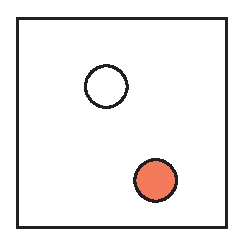
\includegraphics[width=1.5in]{sample.eps}
%  \caption{Lookit! Lookit!}
%}

%% Abstract section.
\abstract{ This article describes ``Obvious'': a meta-toolkit that
  abstracts and encapsulates information visualization toolkits
  implemented in the Java language. It intends to unify their use and
  postpone the choice of which concrete toolkit(s) to use later-on in
  the development of visual analytics applications.  We also report
  on the lessons we have learned when wrapping popular toolkits with
  Obvious, namely Prefuse, the InfoVis Toolkit, partly Improvise, JUNG
  and other data management libraries.  We show several examples on
  the uses of Obvious, showing how the different toolkits can be
  combined, for instance sharing their data models.  We also show how Weka, a
  popular machine-learning toolkits, has been wrapped with Obvious and
  can be used directly with all the other wrapped toolkits. 

  We expect Obvious to start a co-evolution process: Obvious is meant
  to evolve when more components of information visualization systems
  will become consensual. It is also designed to help information
  visualization systems adhere to the best practices to provide a
  higher level of interoperability and leverage the domain of visual
  analytics.
}



%% ACM Computing Classification System (CCS). 
%% See <http://www.acm.org/class/1998/> for details.
%% The ``\CCScat'' command takes four arguments.

\CCScatlist{ 
  \CCScat{K.6.1}{Management of Computing and Information Systems}%
{Project and People Management}{Life Cycle};
  \CCScat{K.7.m}{The Computing Profession}{Miscellaneous}{Ethics}
}

%% Copyright space is enabled by default as required by guidelines.
%% It is disabled by the 'review' option or via the following command:
% \nocopyrightspace

%%%%%%%%%%%%%%%%%%%%%%%%%%%%%%%%%%%%%%%%%%%%%%%%%%%%%%%%%%%%%%%%
%%%%%%%%%%%%%%%%%%%%%% START OF THE PAPER %%%%%%%%%%%%%%%%%%%%%%
%%%%%%%%%%%%%%%%%%%%%%%%%%%%%%%%%%%%%%%%%%%%%%%%%%%%%%%%%%%%%%%%%

\begin{document}

\firstsection{Introduction}

\maketitle

%% -*- mode: LaTeX; -*-

Over the past few years, several information visualization (InfoVis)
toolkits have flourished in various languages such as
Java~\cite{Discovery2,InfoVis, Prefuse, jung2003, Improvise},
C++~\cite{Tulip,ADVIZOR}, Flash/Flex~\cite{Axiis,flare} or
JavaScript with HTML5~\cite{thejit,Protovis} to name a few.  When starting
a visual analytics (VA) project, the choice of the toolkit is a major
initial decision and the resulting proliferation of toolkits can be confusing
for VA software developers who know that an
inappropriate choice can lead to unanticipated limitations during the
development of the application.

Historically, this proliferation of toolkits can be explained by
several factors: each created toolkit addresses a specific set of
problems, is designed with a specific application domain in mind, or
simply offers different tradeoffs.  However, it results in dispersion
in terms of capabilities since each toolkit has unique and useful
techniques for visualization and interaction.  For example, the
Prefuse~\cite{Prefuse} and JUNG~\cite{jung2003} toolkits offer several
graph layout algorithms whereas Improvise~\cite{Improvise} supports
very sophisticated coordinated views with limited graph capabilities.

The choice of an InfoVis toolkit should be made
early in the software development process because it affects not only the visualization techniques but
also the data structure to work with.  For an application dealing with
small quantities of data, copying data from one structure to another
is possible in interactive time but not for VA
applications that usually manage data sets too large to be duplicated
at all.  Therefore, most data-management and analysis will be made on
data structures compatible with the visualization and tied to the
visualization toolkit.

%\jo{changed language in the following paragraph to emphasise that this is a consequence of a lack of meta-toolkit/interface rather than advice.}

Once the choice is made, any missing components have to be added
specifically to the toolkit: if a special data manager is required
(e.g., reading a particular data format), it has to be implemented
specifically for the data structure managed by the toolkit. Any analysis
not supported by the toolkit requires the authoring or adaptation of
analytical toolkit components. Likewise, if visualization techniques
are required that are not supported by the chosen toolkit they must
be added, creating a strong dependency that usually prevents changes
of toolkit later-on in the development.

The effort required by one application to implement the missing
components cannot easily be reused in other applications that are based on another
toolkit.  Therefore, important resources are wasted for the re-implementation of
data converters, analysis modules, and visualization techniques. 

To address this proliferation problem, this article introduces
\emph{Obvious}: a meta-toolkit that abstracts and encapsulates InfoVis
toolkits implemented in the Java language as a way to unify their use
and postpone the choice of which concrete toolkit(s) to use later-on
in the development process.  Obvious is mainly targeted at VA software
developers, but also  library or toolkits developers if they want to
promote sharing of data managers, converters, or algorithms not
restricted to one toolkit.

\noindent This article presents three contributions:
\begin{enumerate}[noitemsep,topsep=0pt]
\item it describes the design and implementations of Obvious,
\item it reports some lessons learned when wrapping existing toolkits
  with Obvious, and
\item it presents rationales for the social process we started and
  want to follow for the future of Obvious.
\end{enumerate}

\noindent The main benefits offered by Obvious are:
\begin{enumerate}[noitemsep,topsep=0pt]
\item it improves the reusability of code and components;
\item it improves the interoperability of code, data models and
  visualizations;
\item it defers the choice of which concrete toolkits to use to a
  later stage of the VA development;
\item it enforces a better separation of concerns in VA
  applications so that the data models can be specified independently
  of the visualizations and views;
\item it allows toolkit and library developers to easily integrate
  their tool into the rich environment of Obvious-compatible systems;
\item it clarifies issues with notification and allows VA to scale up using a standard architecture; and
\item it specifies a set of interfaces and a stable vocabulary which
  simplifies learning.
\end{enumerate}

\begin{comment}
Obvious is implemented in a modular way with an abstract core module
and additional specific bindings, implemented for several toolkits:
the Infovis toolkit~\cite{InfoVis}, Prefuse~\cite{Prefuse},
Improvise~\cite{Improvise} and Jung~\cite{jung2003}.  These bindings
have been used to build some proof-of-concepts examples combining
different toolkits and also to create complete systems used by ongoing
research projects such as~\cite{BENZAKEN:2011:INRIA-00532552:1}.

During the development of bindings, we have seen important design
questions emerge regarding the interpretation of the reference model;
we report them here to help clarify the InfoVis reference model and
trade-offs in its implementation.

In addition, Obvious allows developers to eliminate the crucial choice
of the toolkit and to avoid rewriting existing functionalities such as
file import and export modules, as well as analytical algorithms. The
following use case shows it is now possible to combine toolkits.  For
example, they can choose a data model from JUNG toolkit for a graph,
then query it with Prefuse predicates, use a layout introduced in
Infovis toolkit to display it and still used network algorithms
introduced in JUNG.  With obvious, there are no more design restrictions
imposed by an initial choice for developer.


%\subsection{Goals and Social Process}

Obvious is not another toolkit, it is a set of interfaces that
abstract the services provided by InfoVis toolkits
implemented according to the InfoVis reference
model~\cite{ChiRefModel,ReadingsIV}.  Obvious has been specified
during a workshop gathering several major authors of
toolkits~\cite{vismaster2008}; its interfaces have reached a consensus
at the time of the workshop among the developers.  However, they do
not cover all the parts of the reference model evenly.  The data
component is much more precisely defined than the visualization and
view components. 

In the related work section, we describe several models that have been
used to standardize software 

%\subsection{Targeted uses}

A typical scenario of Obvious would be the design of
VizTree~\cite{lin01}, a VA application for monitoring
massive time-series.  VizTree encodes very long time-series of a
continuous value as a suffix tree; the details of this encoding being
beyond the scope of the paragraph scenario.  The associated tree
visualization has been implemented by specialists of data-mining and
leaves room for improvements in term of visualization and
interaction.  Using Obvious, the authors would first connect their
computed data structure to the data model of Obvious. There are two
ways of doing that: use the Obvious data-model directly or use the
native data-model implemented for mining the time-series and wrap it
with an implementation of the Obvious data-model. Both are possible
and will be chosen according to the amount of work and flexibility
offered by one option or the other. Once an Obvious data-model is
available, the authors of VisTree can start exploring which toolkit
will provide them the best support for their visualization. They can
choose among the InfoVis Toolkit, Prefuse and JUNG to visualize tree
data. Once the best one has been chosen, the interaction can be
crafted either on top of the abstraction provided by Obvious - to keep
the option of switching the final implementation - or using the native
toolkit controls to keep a tighter control of the interface. If
desired, the interface can also be improved by adding other
visualizations associated with the computation of the prefix tree or
of statistics associated with the data. If multiple-coordinated views
are required for that, Improvise visualization and views can be added
to the interface using the same data model. In that scenario, Obvious
has enabled data-mining researchers to focus on their skills and to
use state-of-the-art visualization components at a later stage of the
development of their application.

Another scenario [DDupe]

Yet another, more futuristic scenario: porting a new visualization type to multiple toolkits
or allowing cross-toolkit brushing interaction.

\end{comment}

The article is organized as follows: in section 3, after the related
work section, we describe the design of Obvious. Section 4 reports on
the wrapping of several toolkits and components with Obvious. Section
5 shows examples of Obvious in action to assess its
usefulness. Section 6 discusses the social process we have used and
how we envision the evolution of Obvious before concluding.


\section{Related Work}

Obvious is a set of interfaces and extension classes for wrapping
around existing information visualization toolkits.  It generalizes
and extends the standard architecture as defined in the Information
Visualization reference model to try to abstract all the existing
implementations.  In this section, we list some major existing
toolkits and explain what they share and how they differ.  In the
second section, we describe the most common standardization processes
for software systems.

\subsection{Visualization Toolkits}

Pretty much all existing information visualization toolkits follow the
InfoVis reference model initially specified by Ed Chi and refined by
Card, Mackinlay and Shneiderman~\cite{ChiRefModel,ReadingsIV} and has
been described as a design pattern in~\cite{DesignPatternsIV}.  The
model defines three stages: \emph{DataSet} or \emph{Data Tables},
\emph{Visualization} or \emph{Visual Structure} and \emph{View}
(Figure~\ref{fig:refmodel}).  One of its main benefits is that it
explicitly represents interaction, in contrast to older visualization
models.  Several articles have described the concrete design of an
information visualization toolkit.  We report here on the common and
the specific parts.

\begin{figure}
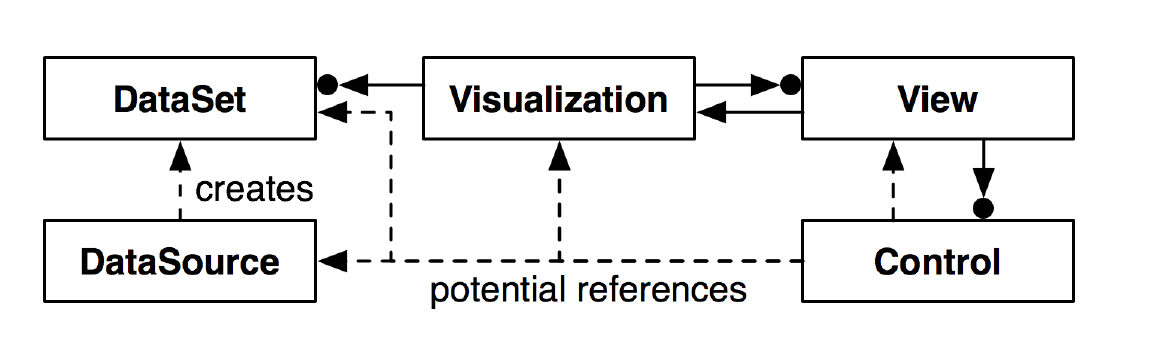
\includegraphics[width=\columnwidth]{figures/refmodpat}
\caption{The Information Visualization Reference Model~\cite{DesignPatternsIV}}
\label{fig:refmodel}
\end{figure}


The InfoVis Toolkit~\cite{InfoVis} is based on an \emph{in-memory
  database manager} where data is organized in columns --- contrary to
most persistent relational databases --- to improve the memory
footprint and allow addition of new attributes that are needed to
manage the interaction (e.g. selection or filtering) and to hold
attributes computed on demand.  The main challenge being the support
of interactive performance for rendering and dynamic queries with a
small memory footprint.  The visual structure is managed using a
\emph{monolithic} architecture~\cite{Polylithic}: each visualization
technique is implemented as a specific class
(e.g. ScatterplotVisualization, ParallelCoordinatesVisualization,
TreeVisualization) that performs the mapping between the data set and
the graphics items to render.  Finally, the view component is the same
for each of the visual structures and takes care of scrolling,
zooming, overlaying magic lenses (e.g. Fisheye or Magic Lenses).  A
\emph{notification mechanism} implements the communication between the
data tables and the visual structure: each time a data table is
modified, it notifies all the registered handlers of the details of
the modification. The interaction is managed by \emph{Interactor}
objects that are associated with the visual structures; the views are
generic and forward interaction managements to the Interactors.  One
specific feature provided by the InfoVis Toolkit is layering:
visualization can be composed on top of each others.  Composite
visualizations are useful to build complex visualization by breaking
them into simple parts. For example, node-link diagrams are split into
links managed as a layer and nodes as another.  Magic lenses and
Fisheyes are also managed as layers on top of other visualizations.

Prefuse~\cite{Prefuse} also relies on an in-memory database with
notification but implements the visual structure using an extension of
the data model (a visual table derives from a data table).  It then
transforms the data into a \emph{polylithic} graphic structures
whereas all the other toolkits use a \emph{monolithic} architecture.
In a polylithic architecture, there is only one component in charge of
all the visual structures.  A visualization object is responsible of
managing a visual structure: it contains visual tables that augment
data tables with graphic attributes (shape, color, etc.)
Visualizations are in charge of computing the layout (assigning a
position and shape to visual items), the graphic attributes and
animations.  Visualizations use a \emph{Renderer} object to actually
display visual items.  Users can control which renderer is used
depending on the visualization and the object itself.  In Prefuse,
data managers, visual managers and views are generic, offering a very
clean interface to the application programmer.  However, as noted by
Bederson at al.~\cite{Polylithic}, polylithic toolkits have a steeper
learning curve than monolithic ones because the polylithic components
do not work out of the box, they always need to be configured.  To
address this issue, Prefuse comes with code samples that simplify the
initial setup.

Building upon their experience in the Prefuse toolkit~\cite{Prefuse},
Heer et Agrawala~\cite{DesignPatternsIV} have derived software design
patterns that are common to information visualization applications and
toolkits. 

Improvise~\cite{Improvise} relies on an in-memory database with
notification that is row-oriented and its visual structures are
monolithic.  The main characteristic of Improvise lies in its
management of coordinated views.  To this aim, it relies on several
design patterns not supported by Prefuse; compared to the other
information visualization toolkits, it adds a coordination component
that is central and extends the notification mechanism implemented
by the InfoVis Toolkit or Prefuse.

Discovery~\cite{Discovery1,Discovery2,Discovery3} shares most of its
characteristics with Prefuse: it uses an in-memory, column-oriented
database and a polylithic graphic model. Its two main features are 1)
the absence of a scene graph, replaced by a dataflow pipeline made of
short operations called \emph{functors} that renders directly from the
data-model, and 2) a deferred notification strategy to allow data
editing.

%% \jo{I'm not sure I am convinced of the assertion in the following
%%   paragraph. The three toolkits above are described in some detail,
%%   not all of which is relevant to other toolkits. Perhaps we should
%%   instead abstract their distinct design characters. e.g. Row-oriented
%%   vs column oriented; in-memory vs cached database management;
%%   monolithic vs polylithic etc. The point being that while they all
%%   attempt to achieve similar general aims, their lower-level approach
%%   to doing so requires different programming approaches, hence the
%%   need for Obvious.}

Other information visualization toolkits can mostly be described using
the four toolkits above, even if they use a different programming
language.  Tulip~\cite{Tulip} is a graph-oriented toolkit programmed
in C++ that uses data tables for vertices and edges, like the InfoVis
Toolkit and Prefuse.  It implements several complex graph layout
algorithms and uses OpenGL for its rendering but the conceptual
architecture is table-based and monolithic.  Therefore, information
visualization toolkits share a global organization, they all implement
an in-memory database with two variants (row-based or column-based), a
visual structure with two variants (monolithic or polylithic) and
several specific features.  Even if some choices made by toolkits
designers were carefully decided, other were probably made without
being aware of the alternatives.  Combining the best possible features
for a next-generation toolkit might be tempting but there are still
tradeoffs that cannot be solved.  For example, the power of
coordinated and linked views offered by Improvise comes at the cost of
maintaining caches that should be flushed when the data change so
there seems to be a tradeoff there that still needs research to be
solved.

There are also lower-level toolkits that can be used to build visual
analytics applications.  Two popular families are graphics libraries
and graph libraries.

%% \jo{I'm not sure what point is being made here with the discussion of
%%   lower level visualization toolkits. Are we asserting that the
%%   standardization implied by Obvious is also appropriate for lower
%%   level approaches to VA software construction? If so, we need to
%%   identify what is lacking in an approach without Obvious as well as
%%   demonstrating (later on in the paper) that implementing the Obvious
%%   interfaces in lower level visualization environments is both
%%   practical and beneficial. An interesting test case might be
%%   \emph{Processing} (processing.org). This is, compared to the other
%%   examples cited, a very low level approach to visualization software
%%   development. However, it is designed for rapid-prototyping, and if
%%   it could be easily integrated with Obvious it might provide a nice
%%   example of how early prototypes could be transformed into more
%%   robust applications using Obvious as the bridge. I'd be happy to
%%   write some words on this if you think it fits well with the theme of
%%   the paper.}

\subsection{Graphics Libraries}

Visual analytics applications can manage their own data structure and
take care of the mapping from data to visualization on their own.  At
this point, they can use \emph{scene-graphs} or \emph{direct-graphics}
libraries.  

Scene-Graph toolkits can manage the visual structure and view as
described in the reference model.  They are focused on computer
graphics and interaction: they only deal with the visual structure and
view.  Piccolo and Jazz~\cite{Polylithic} are popular 2D scene-graph
managers that have been used to create several information
visualization applications (e.g.~\cite{SpaceTree,Geneaquilt}.) An
early version of Piccolo has also been used as graphics engine for the
Cytoscape graph visualization system~\cite{Cytoscape} but dropped for
performance reasons.

High-performance information visualization applications use
scene-graph optimization techniques to speed-up the rendering of
scenes.  Tulip~\cite{Tulip} and Gephi~\cite{Gephi} maintain a spatial
indexing structure to avoid rendering objects that are not visible.

Although scene-graph technologies are mature and used in a wide
variety of graphics applications such as games, virtual-reality
applications and scientific visualization systems, they are not always
adequate for information visualization systems because they require
the explicit specification of geometry and graphic attributes for each
displayed objects.  Very often, information visualization can quickly
compute graphic attributes and even geometry from data attributes.
For example, the position of an item using a scatterplot visualization
is computed using a simple affine transformation the data attributes
using for the X and Y dimensions.  There is no need to store the
computed values when computing them on the fly is very cheap.  The
same is true for color etc.  Copying and storing this information is
costly in terms of time and memory.

Direct-graphics libraries such as \emph{Processing} or \emph{OpenGL}
can also be used to implement the visualization technique while
drawing for rapid prototyping or high-performance reasons.

[Add a section on Processing]

Still, when separating the data-model from the visual model,
scene-graph managers offer more flexibility than information
visualization systems for complex graphics and sophisticated
interaction.  This is why several information visualization systems
still use them.

% say something about the fact that scene-graph toolkits are
% classically for 3D scenes.

\subsection{Graph Libraries}

While most table-based visualization toolkits rely on an in-memory
database, several graph-based visualization systems manage their
data-structures using a model inspired from graph-theory where
topology is the main focus and data associated with graph entities is
less important.  This is the case for the JUNG library~\cite{jung2003}
or the Boost Graph Library (BGL)~\cite{BGL}, as well as for the graph
library used by Cytoscape~\cite{Cytoscape}.

These libraries support graphs as set of vertices and edges (the
topological entities) that can be associated with arbitrary data.
This data is just stored by the graph entities as a convenience for
the application: the library does not implement any integrity check
between data and graph entities.  In contrast, the InfoVis Toolkit,
Prefuse and Tulip maintain a close consistency between graphs and data
tables: removing a data table entry associated with a graph entity
(vertex or edge) also removes the entity from the graph structure.

Thus, there is no clear consensus on how a graph data structure should
be managed internally; the design choices are quite different
depending on the communities such as graph theory, information
visualization, database and semantic web.


\subsection{Standardization Processes}

Standardization is a well established habit in the software community;
several standardization models have been used in the past and these
models tend to evolve due to the growing pace of software development
taking place nowadays.

Standards have been specified by national and international
organization such as the International Organization for
Standardization (e.g. ISO, ASCII), non-profit organizations (e.g. the
Unicode Consortium or OMG), consortia of public or private
organizations (e.g. the World Wide Web Consortium (W3C)). Closer to
the information visualization community, ``The Open Geospatial
Consortium (OGC)\footnote{\url{http://www.opengeospatial.org}} is an
international industry consortium of 423 companies, government
agencies and universities participating in a consensus process to
develop publicly available interface standards.''

\jdf{More to come..}


\section{Design of the meta-toolkit}

%\input(design)

\section{Examples}

Put examples here.

\section{Conclusion}

Put conclusion here. 

%% if specified like this the section will be ommitted in review mode
\acknowledgements{
The authors wish to thank A, B, C. This work was supported in part by
a grant from XYZ.}

\bibliographystyle{abbrv}
%%use following if all content of bibtex file should be shown
\bibliography{obvious}
\end{document}
